% |||||||||||||||||||||||||||||||||||
% |||||| 5.4 Simulation setups ||||||
% |||||||||||||||||||||||||||||||||||

% -------------------------------------
% labels: \label{[type]:PT:sims:[name]}
% -------------------------------------

% ¨¨¨¨¨¨¨¨¨¨¨¨¨¨¨¨¨¨¨¨¨¨¨¨¨¨¨¨¨¨¨
% LOCAL MACROS:
\newcommand{\epsA}{\ALIASepsA}
\newcommand{\epsB}{\ALIASepsB}
\newcommand{\epsC}{\ALIASepsC}
% ¨¨¨¨¨¨¨¨¨¨¨¨¨¨¨¨¨¨¨¨¨¨¨¨¨¨¨¨¨¨¨



% The simulations that were performed in this project and are referenced in the coming discussions are listed in~\cref{tab:PT:sims:sim_setups} for reference. 

% \phpar[simulation details]


% \begin{description}
%     \item[type-0]\label[it]{it:results:something:type0} Use~\cref{eq:PT:gwas:achi_IC_type0} for $\chi$ and its conformal time derivative for $\dot{\chi}$ at some time shortly after $\redshift_\ast$
%     \item[type-$\star$]\label[it]{it:results:something:typestar} Use tweaked initial conditions for field,  
% \end{description}

% \comment{Reasoning behind choices of parameters:}




% \begin{description}
%     \item[Box size:] On one hand, we want the comoving box to be large so that the domain wall thickness $\delta\ped{dw}$ is much smaller than the box size $L_\#$ and the separation between the main wall and its counterpart (the ``anti-wall'') are fare away from each other. On the other hand, to resolve the Compton wavelength $L\nped{C}$, we require $\Delta_\# \leq \lambda\nped{C}$ and in turn $N_\# \geq L_\#/L\nped{C}$.
%     % \item[Compton wavelength] is \emph{not} resolved. On one  
%     \item[Initial time:] The normal quasi-static $\tanh$-profile (\cref{eq:PT:symm_dws:chi_w_quasistatic_FLRW}) approximates the initial configuration to $\breve{\chi}_\ast\to0$ and $\breve{\chi}'_\ast \to \infty$, which does not actually work out. With the analysis in~\cref{sec:PT:symm_dws:asymptotic} we can impose suitable initial conditions so that the field rolls into the minima in the most effective way. However, this affects the expression for the domain wall surface tension and \blahblah 
% \end{description} 


% The code automatically outputs scalar quantities like extremal values of $\chi$ and $q$, as well as their box-averaged values. Besides this, we request two-dimensional snapshots of the field in question at every-something time step. %For example, %to get the full asymmetron field $\chi$, we 
% we request 
% The files produced are of Hierarchical Data Format (HDF5), and each of them contain field values at $N_\#^2$ points. For the asymmetron field, this means at all coordinates $\lcoord{j}, \lcoord{k}$ \blahblah 


 % $\langle \chi^2, q^2 \rangle$, box-averaged,  squared scalar field v at every time step. 



Below, we describe the reasoning behind the choice of parameters. As a starting point, we consider the fiducial set of symmetron parameters $a_\ast =0.33$, $\xi_\ast = 3.33\times 10^{-4}$ and $\beta_\ast = 1$, following~\citet{christiansenCosmologicalSimulationsPhase2024}, that will be defined below (\cref{eq:PT:sims:mapping_symmetron_params}). This gives Compton wavelength $L\nped{C}\approx 1~\Mpch$ and asymptotic wall thickness $\delta_\infty = \sqrt{2} L\nped{C}\sim \sqrt{2} ~\Mpch$. %
%We refer to this as $\vec{\theta}_\ast\ap{fid}=(0.33, 3.33\times 10^{-1}, 1)$.
Simulations are initiated and broken at redshifts $\redshift\ped{i}$ and $\redshift\ped{f}$, respectively.

\subsubsection{Simulation box}
    % In the toy model, we are considering ``infinitely'' broad domain walls with vanishing thickness. We need therefore a simulation box of size that is comparable to the universe, 
    % Size of universe ~ 5000 Mpc/h0

    We use a comoving simulation box size that is comparable to the size of the universe---order $\mathscr{O}(\mathrm{Gpc}/h_0)$---so that $\delta\ped{w}\ll L_\#$ and the separation between the walls is $\sim \wallsep \equiv  L_{\#}/2$. If we want to resolve the Compton wavelength, this requires $N_\# \geq L_\#/L\nped{C} \gtrsim \mathscr{O}(10^3)$. However, since we are modelling the entire formation, conventional walls (\cref{eq:PT:symm_dws:chi_w_quasistatic_FLRW}) will initially be infinitely thick and therefore interact with each other. 

    % On one hand, we want the comoving box to be large so that the domain wall thickness $\delta\ped{dw}$ is much smaller than the box size $L_\#$ and the separation between the main wall and its counterpart (the ``anti-wall'') are far away from each other. On the other hand, to resolve the Compton wavelength $L\nped{C}$, we require $\Delta_\# \leq L\nped{C}$ and in turn $N_\# \geq L_\#/L\nped{C}$.

    We will provide the time step sizes %$\Delta_\tau^{(\mathrm{})}$
    in terms of a Courant factor $C\ped{f}=\Delta_\tau/\Delta_\#$ for the external loop and a number $N_\phi=\Delta_\tau/\Delta_\tau^{(\phi)}$ that sets the number of times the asymmetron field solver is used per cycle. \comment{Bad explanation\dots}

\subsubsection{Initial configuration}

    The normal quasi-static $\tanh$-profile (\cref{eq:PT:symm_dws:chi_w_quasistatic_FLRW}) approximates the initial configuration to $\breve{\chi}_\ast\to0$ and $\breve{\chi}'_\ast \to \infty$, which does not actually work out. %    
    Since $\redshift_\ast=1/a_\ast-1 = 2 + 1/33 > 2$, choosing initial redshift $\redshift\ped{i}=2.00$ leaves wiggle room enough to get simulations started with spatially separated walls. In other words, with $a_\ast=0.33$ and $\redshift\ped{i}=2.00< \redshift_\ast$, there is a tiny slot between SSB and initialisation ($\redshift_\ast-\redshift\ped{i} \approx 0.03$) that we do not simulate.
    
    On the other hand, with the analysis in~\cref{sec:PT:symm_dws:asymptotic} we can impose suitable initial conditions so that the field rolls into the minima in the most effective way. We need to keep in mind that this affects the surface tension and wall width.
    %  However, this affects the expression for the domain wall surface tension and \blahblah 



\subsubsection{Symmetron parameters}
    The code uses phenomenological parameters $(a_\ast, \xi_\ast, \beta_\ast)$ to define the symmetron model. The mapping to Lagrangian parameters $(\mu, M, \lambda)$ is~\citep{christiansenAsevolutionRelativisticNbody2023}:
    \begin{subequations}\label{eq:PT:sims:mapping_symmetron_params}
        \begin{align}
            a_\ast &=  \pclosed{\frac{\rho\ped{cr0} \Omega\ped{m0}}{\mu^2 M^2}}^{1/3},\\
            \xi_\ast &= \frac{H_0}{\sqrt{2}\mu}, \\
            \beta_\ast &=\frac{M\nped{Pl}}{M^2} \frac{\mu}{\sqrt{\lambda}}.
        \end{align}
    \end{subequations}
    $a_\ast$ is the cosmic scale factor at symmetry break, as before, $\xi_\ast= H_0 L\nped{C}$ is the Compton wavelength per Hubble length, and $\beta_\ast$ measures the strength of the fifth force (see~\cref{eq:cosmo:quintessence:framework:fifth_force}). %
    For $\kappa>0$, the parameter $\beta_\ast$ is modified s.t.~$\beta_\ast \to \bar{\beta}= (\beta_+ + \beta_-)/2$, and you get an additional parameter $\Delta \beta = \beta_+- \beta_-$. Formal definitions are found in~\citet{christiansenAsevolutionRelativisticNbody2023}. % For the sake of completeness,


\subsubsection{Nature of wall perturbation}
    For the linear theory to hold, we need $\epsast \ll L$ and $pL \gg 1$ where $L$ is a length scale, earlier taken to be $L\sim \tau_\ast$. For the prototype, we add that $\abs{\varepsilon(\tau)} \gg \delta\ped{w}(\tau)$ for $\tau\in[\tau\ped{i}, \tau\ped{f}]$ for obvious reasons. %, and choose $L\sim L_\#$. % 
    We choose to only perturb one wall so that the time of collision between massless particles propagating from one of the walls is at $ \tau\ped{i} + \wallsep$~\lcomment{Is this true? Maybe col. time is double?}, $\wallsep= L_\#/2$.\footnote{
        Perturbing both walls would give collision time $\tau\ped{i} + L_{\#}/4$.
    } %
    We would like $\epsast \ll \wallsep$, but with a quick look at~\cref{fig:pertwalls:mywalls:demo_analytical_epsilon} we can assume that this would require a very high spatial resolution. As a result, we choose to exaggerate the initial perturbation amplitude and risk higher-order effects. %\verb|..|
    %\lcomment{Maybe give a length scale?}

    % A typical length scale of our setup is perhaps $L/#$; the separation between the two walls. This gives 

    In every simulation, we adjust for the time gap between SSB and initialisation %
    % $\redshift_\ast$ and $\redshift\ped{i}$ 
    by using $\epsA(\tau\ped{i})$ and $\epsA[\dot{\varepsilon}](\tau\ped{i})$ from~\cref{eq:pertwalls:mywalls:eps_s_complete_MD}.


    % First of all, we restrict $\epsast < L_{\#}/4$.





\subsection{Toy-model catalogue}

   


    We present results in~\cref{chap:results} from the eight simulations that are listed in~\cref{tab:PT:sims:sim_setups}, with supplementary visualisation in~\cref{fig:PT:sims:initial_configs}. %
    We largely use~\citet{christiansenAsimulationDomainFormation2024} to help make parameter choices. 
    Every simulation---labelled \simnum{0},~\simnum{1},\dots,~\simnum{7}---uses a 4th order Runge-Kutta solver. 
    We use simulation~\simnum{1} as a starting point and change one or two parameters at a time for subsequent experiments. The middle wall is unperturbed in simulation~\simnum{0}, and this particular experiment works as a sort of benchmark to separate the wall displacement effect. 
    Each simulation is associated with a characteristic colour (see~\cref{tab:PT:sims:sim_setups}) that will distinguish it in figures to come.

    % ------------------------------
    % ----------- FIGURE -----------
    \begin{figure}[ht]
        \centering
        %
        \begin{subfigure}[t]{0.62\linewidth}
            \centering
            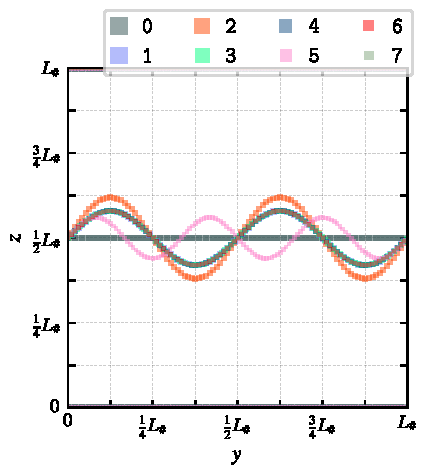
\includegraphics{Methodology/initial_perturbations.pdf}
            \caption{Schematic of the initial wall position in the $yz$-plane for each simulation. Note that~\simnum{1},~\simnum{3},~\simnum{4} and~\simnum{7} are overlapping.} %in the simulations described in~\cref{tab:PT:sims:sim_setups}.}
            \label{fig:PT:sims:intital_perturbations}
        \end{subfigure}
        ~
        \begin{subfigure}[t]{0.32\linewidth}
            \centering
            \includegraphics{Methodology/initial_config.pdf}
            \caption{Initial redshift, and asymptotic scalar and velocity field values.}
            \label{fig:PT:sims:initial_config}
        \end{subfigure}
        %
        \caption{Visual representation of initial configurations listed in~\cref{tab:PT:sims:sim_setups}.}
        \label{fig:PT:sims:initial_configs}
    \end{figure}
    % ------------------------------


    \begin{table}[h]
        \import{tables/Methodology/}{sim_setups.tex}
        \caption{Details about each simulation addressed in~\cref{part:findings}. Each simulation is labelled \simnum{0}--\simnum{7}. See~\cref{sec:PT:sims,sec:PT:gwas} for description of parameters.} %\comment{Should maybe give fiducial set of parameters (sim. \simnum{1}) and only give deviations from this.}}
        \label{tab:PT:sims:sim_setups}
    \end{table}


    % \comment{Some extra simulations for convergence testing!}

    An additional, completely homogeneous simulation (no walls present) is run with the same background as simulation~\simnum{1}, except that the symmetron initial conditions are optimised as described~\cref{app:stablesym} with $\redshift\ped{i}=2.03$ and $\redshift\ped{f}=1.6$. %In particular, 
    
    




% \subsection{Caveats}
%     We address some of the most obvious problems and paradoxes when simulating these domain walls.
%     %
%     \begin{description}
%         \item[Box size:] On one hand, we want the comoving box to be large so that the domain wall thickness $\delta\ped{dw}$ is much smaller than the box size $L_\#$ and the separation between the main wall and its counterpart (the ``anti-wall'') are fare away from each other. On the other hand, to resolve the Compton wavelength $L\nped{C}$, we require $\Delta_\# \leq \lambda\nped{C}$ and in turn $N_\# \geq L_\#/L\nped{C}$.
%         % \item[Compton wavelength] is \emph{not} resolved. On one  
%         \item[Initial time:] The normal quasi-static $\tanh$-profile (\cref{eq:PT:symm_dws:chi_w_quasistatic_FLRW}) approximates the initial configuration to $\breve{\chi}_\ast\to0$ and $\breve{\chi}'_\ast \to \infty$, which does not actually work out. With the analysis in~\cref{sec:PT:symm_dws:asymptotic} we can impose suitable initial conditions so that the field rolls into the minima in the most effective way. However, this affects the expression for the domain wall surface tension and \blahblah 
%     \end{description} 



% $\chi\rvert_{a}$